
\part{DRAFT}

\section{Définitions préliminaires}

Fermetures et ouvertures du canon

Malgré une grande stabilité dans le temps, le canon littéraire est malléable dans ses marges. Bossuet, Buffon


\section{Le canon littéraire et sa construction}

Il existe une approche plus traditionnelle qui étudie le canon littéraire, sa construction et sa pérennité dans le temps. 


\enquote{Le canon renvoie aux textes — ou aux objets — que les institutions académiques établissent comme les meilleurs, les plus représentatifs et les plus significatifs dans les domaines de la littérature, de l’histoire de l’art ou de la musique. Dépositaires d’une valeur esthétique transhistorique, les canons des diverses pratiques culturelles établissent non seulement ce qui est incontestablement grand, mais aussi ce qui doit être étudié comme modèle par ceux qui aspirent à l’une de ces pratiques.}
\footcites{harder_deconstruire_2013} ? ou pollock ?


\section{Littérature}

Littérature
[ref Daniel COUTY, Histoire de la littérature française, p39]
Le terme littérature, dans son acceptation moderne, renvoie à un corpus élaboré, consacré par la tradition, de textes portant la marque de de préoccupations d'ordre esthétique et qui ont (acquis) valeur de modèle. letre ou letreure qualifient eux un apprentissage et une activité, ceux du lettré, du clerc, qui consistent à s'approprier un savoir puisé dans les textes faisant autorité, les auctores, textes sacrés et les écrits des Pères de l'Église
formes littéraires qui s'interrogent sur leurs conditions de production et d'écriture et prétendent à la beauté formelle. 

Ce qu'on appelle littérature = canon
Canon 
Classique

\footnote{Sainte-Beuve, \textit{Réflexions sur les lettres}}

\chapter{La construction du canon littéraire ou l'histoire des remous de l'idée de littérature dans l'enseignement}

\section{L'enseignement scolaire comme matrice du canon littéraire}
Ainsi loin d’être immanente à l’œuvre, la valeur littéraire est relative à un moment socio-historique, en relation avec des institutions littéraires, la critique, et le discours scolaire.

Un bref aperçu de l'histoire de l'enseignement de la littérature peut nous apprendre beaucoup sur les missions de l'enseignement français dans la société, des modèles qu'il utilise pour définir les normes d'expressions.

Dans l'enseignement français du milieu du XIX\ieme siècle, les humanités classiques se définissent d'abord et surtout par une "éducation", une éducation esthétique, rhétorique, mais également morale et civique.

Sujets et programmes permettent de définir les attentes institutionnelles, concernant en particulier le statut de la littérature française, les listes d’auteurs sélectionnés, 

Ce que je voudrais souligner avec cette partie est que l'enseignement scolaire se fonde sur le canon littéraire pour diffuser un modèle de pratique de la communication orale ou écrite. 

Les belles lettres

En effet, la construction politique de la culture nationale est largement dépendante de la culture de ses enseignants. Dépendance du canon à l'institution scolaire (formation et recrutement des professeurs)

\subsection{Histoire de l'idée de littérature dans l'enseignement}
Un bref aperçu de l'histoire de l'enseignement de la littérature peut nous apprendre beaucoup sur les missions de l'enseignement français dans la société, des modèles qu'il utilise pour définir les normes d'expressions. Aussi, l'institution scolaire produit des panthéons d'auteurs et de textes, souvent sous la forme de morceaux choisis [ref JEY] pour éduquer des générations d'écoliers.

sur les mécanismes de production de panthéons d'auteur mais aussi sur les critères de sélection de ces auteurs. 


les humanités ont très vite été investie d'un rôle dans l'histoire de l'enseignement français. 
\footcites{chervel_histoire_1993}

\enquote{De l'honnête homme des âges classiques à l'homme cultivé de l'époque contemporaine, l'individu qu'elle forme, c'est celui qui par la pratique des textes et des auteurs, par le contact avec des civilisations fondatrices, par l'exercice de la traduction, de l'imitation et de la composition, a acquis le goût, le sens critique, la capacité de jugement personnel et l'art de s'exprimer oralement et par écrit conformément aux normes reçues. }\footcites{compere_les_1997}

de à les humanités ont constitué à ériger le socle solide de la culture française formation dédiée à une élite de la population (3\% de la classe d'âge) mais rapproche les générations dans une culture commune. 

[ref Barthes le bruissement de la langue - Réflexions sur un manuel]
\enquote{\textit{L'enseignement de la littérature}, est pour moi presque tautologique. La littérature, c'est ce qui s'enseigne, un point c'est tout.}


\section{Sociologie du prestige littéraire}

Pierre Bourdieu discute de l'importance des contextes d'une oeuvre, qui est nécessairement située dans un espace précis du champ littéraire, défini par les sphères d'influences (auteur, éditeur, lecteur pour faire simple) qui participent à son instauration en tant qu'objet littéraire. 

S'il y a sans doute de nombreuses explications qualitatives à ces deux \enquote{modes de vieillissement}\footnote{\cite{bourdieu_les_1992} p210}(appartenance à un sous-genre littéraire peu prestigieux, ambitions commerciales plutôt que littéraires, ou le contraire pour les classiques, qui doivent au système d'enseignement leur consécration, et donc leur marché étendu et durable), nous sommes persuadés que l'on peut effectuer un diagnostique quantitatif de cette intuition. Ainsi, ce mémoire plonge dans les dynamiques textuelles qui fondent le canon littéraire.

L'idée n'est pas de contredire les recherches en théorie littéraire ou en sociologie \footcites{bourdieu_distinction_2012}\footcites{bourdieu_les_1992} qui démontrent que les mécanismes de prestige littéraire sont fondés sur des facteurs appartenant aux dehors du texte. Ces facteurs sont liés entre autres aux dynamiques de domination à l'oeuvre au sein du champ littéraire. Ce mémoire ne veut en aucun cas occulter les facteurs sociaux ou les logiques commerciales qui régissent la production littéraire dans son ensemble, des écrivains en passant par les éditeurs jusqu'aux lecteurs. 

The creation of the canon is subjective, the result of many individual institutions susceptible to arbitrary, ideo-
logical, random, formal, political, and other motivations.\footnote{J.D. Porter \enquote{Popularity/Prestige}, Pamphlets of the Stanford Literary Lab 17 (2018), url: \url{https://litlab.stanford.edu/LiteraryLabPamphlet17.pdf}. Published in \cite{moretti_canonarchive_2017}}

Shifting Scales\footcites{english_shifting_2016}
How Cultural Capital Works\footcites{piper_how_2016}

Casanova - République mondiale des lettres



\newpage
\section{Stylométrie roulante}

Nous voulons maintenant comprendre, à l'échelle d'un roman, comment se comporte le modèle et ce qu'il détecte dans le récit. Pour cela, nous mettons en place des études en stylométrie roulante. Le processus est assez simple : nous découpons le roman en morceaux de mots, en l'occurrence 500 mots, avec 100 mots partagés entre chaque morceaux, et nous mesurons pour chaque passage le score de la somme des coefficients du modèle statistique. 

\bigskip
\begin{figure}[!ht]
    \centering
    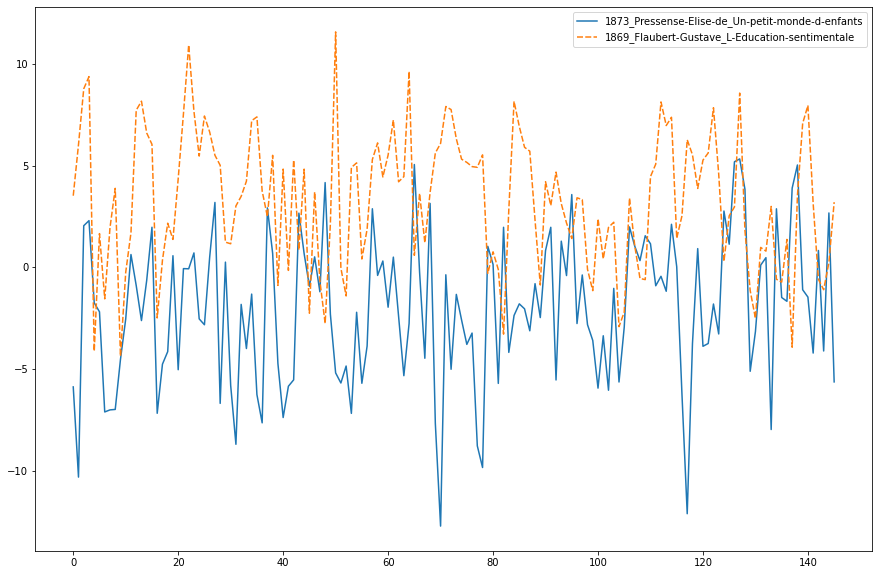
\includegraphics[width=11cm]{img/18_flaubert_signal.png}
    \caption{Signal Canonique dans deux romans}
    \label{signal}
\end{figure}

La figure \ref{signal} représente ce signal dans deux textes : Le premier est canonique, il s'agit de \textit{L'éducation sentimentale}, de Gustave Flaubert. Le second est non-canonique, il est écrit par Élise Pressense et s'intitule \textit{Un petit monde d'enfants}. Le signal des deux ouvrages se distingue assez bien, en orange pour Flaubert et en bleu pour Pressense. Le signal de \textit{L'éducation sentimentale} est assez stable, il oscille entre 0 et 10, et contraste avec celui de \textit{Un petit monde d'enfants}, qui oscille entre 0 et -10. Ces différences s'expliquent notamment par le fait que le roman d'Élise Pressense appartienne à la littérature jeunesse, le modèle le classifie donc \textit{non-canon}. 

Nous mettons en annexe \ref{eds} le passage le plus canonique selon les coefficients du modèle dans \textit{L'éducation sentimentale}. Ce dernier est intéressant puisque Frédéric éperdument amoureux de Mme Arnoux

En annexe \ref{enfants} se trouve le passage le moins canonique du roman \textit{Un petit monde d'enfants}. 

Ainsi, Notre modèle 




Conclusion : 
En essayant de distinguer la fiction de la non-fiction, en trouvant ce qui rend la fiction et le roman uniques en tant que types d'écriture, j'ai tenté de comprendre leur fonction sociale plus large, de répondre à cette éternelle question : " pourquoi la littérature est-elle importante ? D'après les résultats présentés ici, si nous nous concentrons sur les qualités quantitativement distinctes des romans en particulier - sur ce qui les sépare des écrits non fictionnels ou "vrais" - nous pouvons dire que l'importance du roman depuis le XIXe siècle semble être moins une question de réalisme social que de rencontre phénoménologique, une sorte d'immersion sociale dans le monde. Ce n'est pas que ce soit la seule façon dont les romans ont été ou pourraient être significatifs pour les lecteurs. C'est le problème des approches prédictives par rapport aux approches descriptives que j'ai abordé au début - la prévisibilité exclut d'autres possibilités, d'autres qualités qui peuvent être importantes. Les modèles descriptifs identifient simplement quelles caractéristiques diffèrent et de combien, sans présupposer une limite à l'espace des caractéristiques. \footcites{piper_fictionality_2016}



À cet égard, poser une fusion de la lecture humaine et de la machine est une provocation, mais pas une hérésie contre, ou une dégradation du texte littéraire, ni du travail que nous faisons en tant que critiques littéraires. Il s'agit de rendre l'objet littéraire à une ontologie qui a été, et est de plus en plus, la sienne. - une ontologie que nous encadrons aujourd'hui par le langage de données et d'algorithmes, et que les générations précédentes définissaient à travers le langage de la fréquence, de la formule et de l'imitation. Les machines nous aident à trouver les modèles de relation que nous avons toujours su opérer dans la création et la diffusion des styles littéraires, mais que jusqu'à présent nous avons été limités dans notre capacité à reconnaître Piper fictionality aussi ?



Marie Pierre Harder : canon occidental norme et définition de la culture occidentale, mise en cause du statut des classiques dans le cadre nouveau des littératures monde (casanova, weltliteratur, moretti)(re)définition de la littérature comme objet mondial et transnational entraîne-t-elle une(re)définition de la notion et fixation du « canon » littéraire ? définition du littéraire: que devienne les critères de la beauté de l'universalité quand leur bases historiques sont mises en causes + histoire du lexique critique et esthétique canon, classique, ... que sur les conditions sociologiques, idéologiques et culturelles de la production des critères et normes de définition et sélection qui en découlent aussi bien au sein d’un champ littéraire national que dans le cadre de la « République mondiale des lettres » (P. Casanova) Normativité du canon construction d'un partage entre culture populaire et culture classique.

 